\documentclass[finnish,utf8,nonumbib,palatino,kandi]{gradu2}
\usepackage[utf8]{inputenc}
\usepackage[pdftex]{graphicx}
\usepackage{listings}
\usepackage{color}
\usepackage{qtree}

\makeatletter
\ifgradu@pdf
  \usepackage[pdftex,bookmarksopen,bookmarksnumbered]{hyperref}
%\hypersetup{colorlinks,citecolor=blue}

\else
	\RequirePackage[hypertex]{hyperref}
\fi
\makeatother

\title{MVC-arkkitehtuurin toteutus Pyramid web-sovelluskehyksessä}
\setauthor{Toni Juhani}{Haka-Risku}
\yhteystiedot{tojuhaka@gmail.com}
\translatedtitle{Pyramid-framework and MVC-architecture}
\abstract{How does the Pyramid-framework use the MVC-architecture?}
\tiivistelma{Millä tavalla MVC-arkkitehtuuri toteutuu Pyramid web-sovelluskehyksessä?}
\keywords{Pyramid, MVC, Sovelluskehys, Python}
\avainsanat{Pyramid, MVC, Framework, Python}

\definecolor{light-gray}{gray}{0.96}

\lstdefinelanguage{Smalltalk}{
morekeywords={true,false,self,super,nil},
sensitive=true,
morecomment=[s][\color{blue}]{"}{"},
morestring=[d]',
alsoother={_},
style=SmalltalkStyle,
columns=fullflexible,
basicstyle=\ttfamily,
backgroundcolor=\color{light-gray},
xleftmargin=.20in,
showspaces=false,
framexleftmargin=15pt,
tabsize=4
}
\lstdefinestyle{SmalltalkStyle}{
literate={:=}{{$\gets\ $}}2{^}{{$\uparrow$}}1{_}{{$\gets\ $}}2{ä}{{\"a}}2{ö}{{\"o}}2
}

\begin{document}
\preface

Tutkimuksen aiheen valintaan vaikutti työelämässä saatu
 kokemus web-sovellusten kehittämisestä Python-ohjelmointikielellä. Erityisesti
kokemusta on kertynyt Plone-sisällönhallintajärjestelmästä, josta myös Zope- sekä
Grok-sovelluskehys on tullut tutuiksi. Kokemuksen kautta on myös herännyt mielenkiinto
muita tarjolla olevia vaihtoehtoja kohtaan, joista tällä hetkellä uusin on Pyramid. Koska suurin osa Python-pohjaisista
web-sovelluskehyksistä käyttää MVC-arkkitehtuuria, on mielenkiinto herännyt myös itse MVC-arkkitehtuuriin. Tämä johti
kandidaatintutkielman aiheeseen, jossa tarkastellaan MVC-arkkitehtuurin suhdetta Pyramid web"-sovelluskehykseen.

\section{Sanasto}
\begin{description}
    \item[Sovelluskehys] tarjoaa sovelluksen kehitykseen mukaan tason, joka tarjoaa erilaisia kirjastoja yleisimpien ohjelmointiongelmian ratkaisemiseksi. Sovelluskehys on eräänlainen työympäristö, joka helpottaa sovelluksen toteuttamista.
    \item[ZCA] \emph{Zope Component Architecture} on Python-sovelluskehys, joka tarjoaa välineitä komponentti-pohjaisen sovelluksen toteutukseen\cite{ZCA}. 
    \item[Grok] on Pythonilla toteutettu web-sovelluskehys, joka on rakennettu käyttäen pohjana ZTK:ta (Zope Tool)\cite{grok}.
    \item[Zope] on Python-ohjelmointikielellä toteutettu avoimen lähdekoodin web-sovelluspalvelin\cite{zope}.   
    \item[URL] \emph{Uniform Resource Locator} on merkkijono, joka viittaa johonkin tiettyyn resurssiin Internetissä\cite{URL}.
    \item[HTML] \emph{HyperText Markup Language} on merkkauskieli, jolla luodaan dokumentteja, jotka ovat helposti siirrettäviä erilaisten alustojen välillä\cite{HTML}.
\end{description}

\mainmatter
\section{Johdanto}
Toteutuuko MVC-arkkitehtuuri Pyramid-sovelluskehyksessä?

\subsection{Tausta}
Rakentaessamme interaktiivisia sovelluksia, modulaarisilla komponenteilla on paljon etuja. Suunnittelemalla komponentit mahdollisimman erillään toisistaan helpotetaan
sovelluksen ohjalmakoodin hallintaa. Samalla pystytään muuttamaan ohjelmakoodia ilman, että tarvitsee tuntea koko sovelluksen toteutusta\cite[s.2]{Krasner:desc}
MVC-arkkitehtuuri on ohjelmistokehityksessä käytetty rakenne, joka määrää ohjelmakoodin jaottelun kolmeen osaan: Malli(model), Näkymä(view) ja Ohjain(controller). MVC on käytössä monissa sovelluksissa ja erityisesti se on saanut
huomiota web"-sovelluskehyksien toteutuksissa. Sovelluskehyksen tehtävänä on tuoda sovelluksen kehitykseen mukaan
taso, joka tarjoaa erilaisia kirjastoja ratkaisemaan yleisimpiä ongelmia. Monet Python sovelluskehykset kuitenkin luokitellaan MVC-sovelluskehyksiksi\cite{mvcframeworks}, mutta eivät
todellisuudessa toteuta täysin MVC-arkkitehtuuria sellaisena kuin se alunperin olisi tarkoitettu. Näistä yleisimpiä sovelluskehyksiä ovat Python-pohjaiset
ja erityisesti ZCA:n (Zope Component Architecture) omaavat kehykset, kuten esimerkiksi Pyramid ja Grok. Syy sille, miksi
kyseiset sovelluskehykset eivät toteuta MVC:tä täysin, on konkreettisen ohjaimen puute.
Herää kysymys siitä ovatko kyseiset sovelluskehykset MVC-kehyksiä vai eivät? Tämän tutkimuksen tarkoituksena on vastata kysymykseen Pyramid-sovelluskehyksen näkökulmasta.

\subsection{Aiheen rajaus}
Tutkielmassa käsiteltävä aihe on rajattu tarkastelemaan Pyramid web-sovelluskehystä sekä MVC-arkkitehtuuria. Pyramidia
tarkastellaan MVC:n näkökulmasta, joten muihin Pyramidissa käytetyihin tekniikoihin ei oteta kantaa. Pyramidiin on saatavana myös suuret määrät erilaisia lisäosia,
joilla saadaan sovelluskehys muokattua tiettyyn tarkoitukseen.
Lisäksi lisäosat voivat tuoda pyramidiin uusia tekniikoita. Tästä syystä on lähes mahdotonta tutkia MVC:n toteutusta kaikkien tekniikoiden näkökulmasta,
joten tutkielmassa käsitellään ainoastaan Pyramidin alkuperäistä toteutusta ilman lisäosia.

Tutkielmassa selvitetään MVC:n sekä web-sovelluskehyksien taustat ennen varsinaista tutkimuskysymyksen käsittelyä. MVC-arkkitehtuurin esimerkkitoteutukset ohjelmointitasolla sidotaan Smalltalk -ohjelmointikieleen.
Syy kielen valintaan löytyy MVC-arkkitehtuurin historiasta sekä lähekirjallisuuden tarjoamasta materiaalista. Esitellyt ratkaisut
pätevät kuitenkin mihin tahansa muuhun ohjelmointikieleen, joten kielen valinnalla ei tässä tilanteessa ole merkitystä.
 MVC:n tarkastelu Pyramidissa toteutetaan Krasnerin julkaiseman artikkelin pohjalta, jossa käydään kattavasti läpi MVC:n käyttöä ohjelmakooditasolla\cite{Krasner:desc}.  \\
Tutkimuksessa esitetyissä esimerkeissä oletetaan lukijalla olevan perus ohjelmointitaidot hallussa. Joitain tutkimuksessa käytettyjä termejä ei selitetä erikseen, vaan ne löytyvät tutkimuksen sanasto-osiosta.

\section{Kirjallisuuskatsaus}
Kirjallisuuskatsauksessa käydään läpi vaihe vaiheelta, miten lähdemateriaalia kerätään
tutkimusta varten. Lähdemateriaalin haku toteutetaan hakukoneilla, jotka ovat tarkoitettu
erityisesti tieteellisten artikkeleiden etsimiseen. Tässä tutkielmassa käytetyt hakukoneet ovat seuraavat:
IEEE Xplore, ACM Digital Library, Google Scholar sekä joissakin tapauksissa Google:n perinteinen hakukone.

Aluksi muodostetaan kokonaiskuva tuloksista, jolloin silmäillään läpi saatuja artikkeleita. Tässä
vaiheessa tarkoitus ei ole vielä valita mitään pohjaksi tutkimukselle, vaan kerätä informaatiota
siitä millainen lähdemateriaali on tarjolla kokonaisuudessaan. Saaduista tuloksista poimitaan artikkeleita,
jotka sopivat tutkielman aihepiiriin. \\
Seuraavaksi artikkeleista valitaan tutkielmalle pohjakirjallisuus. Tässä vaiheessa artikkelit luetaan huolellisesti
läpi ja varmistutaan siitä, että ne ovat tieteellisesti päteviä tutkielmaa varten. Tutkielmassa esiintyy myös
satunnaisia viittauksia, joita ei ole kirjallisuuskatsauksessa mainittu. Tutkielman pääkirjallisuus kuitenkin käydään läpi kirjallisuuskatsauksessa.

Haussa käytetään seuraavia hakutermejä: "MVC" , "MVC Architecture" ja "MVC-Architecture".  Erityisesti
artikkeleita löytyy MVC-arkkitehtuurin soveltamisesta erilaisissa tekniikoissa. Tarkasteltavat artikkelit rajataan kuitenkin niihin, jotka esittelevät suoraan MVC:tä itseään.

Google Scholarin tuloksista löytyy kaksi artikkelia, jotka sopivat
lähdemateriaaliksi tutkielmaan. Ensimmäinen artikkeleista on John Deaconin kirjoittama artikkeli, joka
tarkastelee lyhyesti MVC:tä\cite{Deacon:1995}. Artikkeli on kuitenkin hyvin suppea, mutta
selittää tiivistetysti MVC:n idean.

Toinen artikkeli on Steve Burbeckin kirjoittama, joka käsittelee MVC:tä sellaisena kuin
sitä käytettiin Smalltalkissa\cite{Burbeck}. Burbeckin artikkeliin viitataan
monissa MVC:tä käsittelevissä julkaisuissa, joten sen arvo tämän tutkielman pohjakirjallisuudessa on vahva.

Seuraavaksi kartoitetaan pohjakirjallisuutta käyttäen ACM Digital Library sekä IEEE XPlore -hakukoneita. Tuloksista löytyy Glenn E.
Krasnerin kirjoittama julkaisu, jossa esitellään MVC:n toteutusta erilaisissa Smalltalk-sovelluksissa. Julkaisusta löytyy useita versioita, joista tässä tutkielmassa käytetään kumpaakin\cite{Krasner}\cite{Krasner:desc}.  Suurimmaksi osaksi viitataan kuitenkin uudempaan julkaisuun. Tuloksien joukosta
löytyy myös paljon MVC:tä soveltavia tutkimuksia, jotka eivät suoraan tarkastele MVC:tä sellaisenaan. Monien MVC-arkkitehtuuria soveltavien artikkeleiden lähdeviitteistä löytyy viittauksia Burbeckin ja Krasnerin artikkeleihin. Tämän perusteella pystytään
toteamaan kyseisten artikkeleiden olevan tieteellisesti päteviä ja tarjoavan kattavan lähdemateriaalin MVC:n pohjaksi. Burbeckin ja Krasnerin kirjoittamien artikkeleiden taustalta löytyy
MVC-arkkitehtuurin kehittäjä Trygve Reenskaug, jonka omia julkaisuja sekä kotisivujen MVC-osiota
käytetään myös lähteenä tutkielmassa\cite{Reenskaug}.

\section {Tutkimuksen rakenne}
Tutkielma aloitetaan käymällä kirjallisuuskatsauksena läpi MVC-arkkitehtuurin käsite sekä sen toteutus ohjelmointitasolla. Kirjallisuutena käytetään
pääasiassa Krasnerin ja Burbeckin julkaisua\cite{Krasner:desc, Burbeck}. Tämän jälkeen käydään läpi Pyramid sovelluskehyksen peruselementit sekä asetetaan
kriteerit, joiden pohjalta MVC:tä tutkitaan Pyramidissa. Kriiteereillä tarkoitetaan ennalta määrättyjä ominaisuuksia, joita Pyramidin tulee toteuttaa MVC:n näkökulmasta. tutkielmassa toteutetaan yksinkertainen laskurisovellus käyttäen pohjana
Krasnerin julkaisussa toteutettua vastaavaa sovellusta\cite{Krasner:desc}. Lopuksi tehdään johtopäätökset tutkielman tuloksista.


\section {MVC}
MVC-arkkitehtuurin perusajatus on erottaa käyttöliittymä sovelluslogiikasta ja
näin tehdä sovelluksesta helposti ylläpidettävä kolmen eri komponentin avulla:
Malli (Model), Näkymä (View) ja Ohjain (Controller). Jokainen komponentti on
erikoistunut sovelluksessa johonkin tiettyyn tehtävään. Mallin tehtävänä on
hallita sovelluksen tilaa ja vastata sen käsittelemästä datasta ohjaimelle ja näkymälle.
Näkymän tehtävänä on taas toteuttaa sovellukselle käyttöliittymä. Ohjaimen tarkoitus on ottaa
vastaan syötteitä käyttäjältä käskien mallia ja näkymää muuttumaan tarvittaessa.

\begin{figure}[h]
\centering
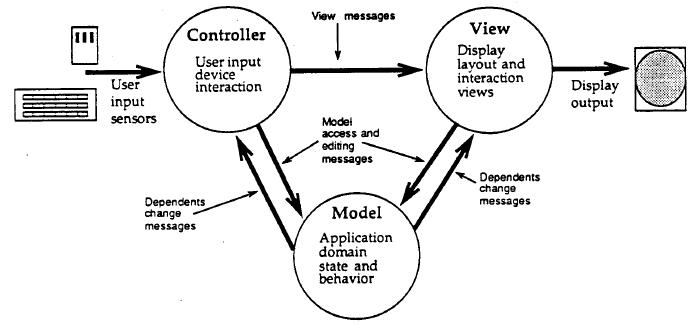
\includegraphics[scale=0.85]{krasner_mvc.jpg}
\caption{Model-View-Controller State and Message Sending\cite[s. 5]{Krasner:desc}}
\end{figure}

Jokaisella komponentilla on oma rajattu tehtävänsä ja ohjelmakoodi tulee jakaa näiden komponentien kesken. Jotta MVC:tä pystyttäisiin käyttämään
tehokkaasti, tulee ymmärtää komponenttien työnjako sekä se kuinka komponentit kommunikoivat keskenään\cite{Burbeck}. \\
Luodessamme MVC-arkkitehtuurin toteuttavia komponentteja, tulee ne periä jostakin abstraktista pohjaluokasta (Model, View tai Controller), joka määrittelee kyseisen komponentin käyttäytymisen MVC:ssä \cite[s. 5]{Krasner:desc}.  Tässä kappaleessa käydään jokaisen komponentin toteutus erikseen läpi käyttäen ohjelmointikielenä Smalltalkia. Lähteenä käytetään Krasnerin julkaisua\cite{Krasner:desc}.

Yleisesti MVC-komponenttien toimintaa kuvaavassa esimerkissä käyttäjältä tulee jokin syöte, jonka sillä hetkellä aktiivinen ohjain ottaa vastaan. Syötteen perusteella ohjain lähettää mallille viestin. Malli puolestaan tekee sille määrättyjä operaatioita muuttaen tilaansa ja lähettää edelleen viestin muutoksestaan kaikille siihen kiinnitettyille riippuvuuksille (näkymät ja ohjaimet). Näkymät
voivat tämän jälkeen kysyä mallilta sen nykyistä tilaa ja päivittää itsensä, jos siihen on tarvetta. Ohjaimet voivat myös muuttaa tilaansa riippuen mallin tilasta\cite[s. 4]{Krasner:desc}.

MVC:n avulla luodaan illuusio siitä, että käyttäjä kommunikoi suoraan mallin kanssa. Todellisuudessa kuitenkin ohjain ja näkymä muodostavat yhdessä rajapinnan sille, miltä malli näyttää ulospäin ja miten sitä käsitellään. Ohjain huolehtii syötteiden vastaanottamisesta ja käsittelemisestä. Näkymä taas huolehtii mallin graafisesta puolesta\cite[s. 11-12]{Reenskaug:tools}. 

\subsection{Historia}

MVC:n esitteli Trygve Reenskaug ollessaan mukana Xerox PARC -tutkimushankkeessa. Ensimmäinen julkaisu MVC:stä
kirjoitettiin vuonna 1978 samassa tutkimuskeskuksessa. Tuolloin julkaisussa esiteltiin kolmen komponentin sijasta neljä
komponenttia: Malli (Model), Näkymä(View), Ohjain(Controller) sekä Muokkaaja(Editor). Muokkaaja on väliaikainen komponentti, jonka näkymä
luo itsensä ja syötelaitteiden välille. Muokkaaja-komponentista kuitenkin luovuttiin käsitteenä ja se sisällytettiin näkymään ja ohjaimeen\cite{Reenskaug}.
Alkuperäinen Xerox PARC:n tuottama raportti MVC:stä oli Reenskaugin vuonna 1979 kirjoittama \emph{THING-MODEL-VIEW-EDITOR}\cite{Reenskaug:1979}. Raportti
esitteli MVC:n komponentteja käyttäen hyväksi esimerkkejä Reenskaugin omasta suunnittelutyöstä. Reenskaug päätyi kuitenkin termeihin \emph{Model-View-Controller} ja julkaisi saman
vuoden lopulla raportin, jossa määritellään lyhyesti jokaisen komponentin tehtävä (\emph{MODELS-VIEWS-CONTROLLERS})\cite{Reenskaug:2007}.

Koska MVC:n historia ja suurin osa MVC:n
alkuperäisistä julkaisuista pohjautuvat Smalltalk -ohjelmointikieleen, joudutaan väistämättä sitomaan MVC:n tarkastelu Smalltalk:iin. Tämä ei kuitenkaan rajoita tarkastelua, koska arkkitehtuurin idea pysyy täysin samana riippumatta ohjelmointikielestä. 

\subsection{Malli (Model)}
Malli pitää yllä sovelluksen tilaa sekä vastaa sovelluksen tallentamasta datasta. Se voi olla esimerkiksi kokonaislukumuuttuja laskuri-sovelluksessa, merkkijono-olio tekstinkäsittelyohjelmassa tai
mikä tahansa monimutkainen olio\cite[s. 3]{Krasner:desc}. Kaikkein yksinkertaisimmassa tapauksessa mallin ei tarvitse kommunikoida ollenkaan ohjaimen ja näkymän kanssa, vaan toimia passiivisena säiliönä datalle.
Tällaisesta tilanteesta on hyvä esimerkki yksinkertainen tekstieditori, jossa teksti nähdään juuri sellaisena kuin se olisi paperilla. Tässä tapauksessa mallin ei tarvitse ottaa vastuuta
kommunikoinnista näkymälle, koska muutokset tekstiin tapahtuvat käyttäjän pyynnöstä. Tällöin ohjain ottaa vastaan käyttäjän syötteet ja voi esimerkiksi ilmoittaa näkymälle muutoksesta, jolloin näkymä
päivittää mallin. Ohjain voi myös päivittää mallin ja ilmoittaa tästä näkymälle, jolloin näkymä voi pyytää mallin sen hetkistä tilaa. Kummassakaan tapauksesssa mallin ei tarvitse tietää ohjaimen ja näkymän
olemassaolosta\cite{Burbeck}.

Malli ei kuitenkaan aina voi olla täysin passiivinen. Se voi myös muuttua ilman, että se tarvitsee ohjaimen tai näkymän käskyä. Otetaan esimerkiksi malli, joka muuttaa tilaansa satunnaisin väliajoina. Koska malli muuttaa itseään, täytyy sillä olla jokin yhteys näkymään, jotta se voi antaa tiedon muutoksestaan\cite{Burbeck}. Datan kapseloinnin ja ohjelmakoodin uudelleen käytön kannalta ei ole kuitenkaan järkevää, että malli on suoraan yhteydessä näkymään ja ohjaimeen. Ohjaimen ja näkymän tulee siis olla riippuvaisia mallista, mutta ei toisinpäin. Näin mahdollistetaan myös se, että mallilla voi olla useita näkymiä ja ohjaimia\cite[s. 4]{Krasner:desc}.

Yleensä mallin tila muuttuu ohjaimista tulleiden käskyjen kautta. Tämän muutoksen tulisi heijastua kaikkiin näkymiin, jotka ovat sidottuja malliin. Tällaisia tilanteita varten kehitettiin riippuvuudet (\emph{dependents}).
Riippuvuuksilla tarkoitetaan listaa niistä ohjaimista ja näkymistä, jotka ovat sidottuja malliin. Mallilla tulee siis olla lista riippuvuuksista ohjaimiin ja näkymiin sekä myös kyky lisätä ja poistaa niitä. Malli ei siis tiedä mitään yksittäisistä riippuvuuksista, mutta pystyy kuitenkin lähettämään itsestään muutosviestejä (\emph{change messages}) listassa oleville ohjaimille ja näkymille. Mallin tuottamat muutosviestit voivat olla minkä tyyppisiä tahansa, joten ohjaimet ja näkymät reagoivat niihin omalla määritellyllä tavallaan \cite[s.2-3]{Krasner}.

Mallille määritellään pääluokka \emph{Model} ja tälle viitemuuttuja \emph{dependents}, joka viittaa yhteen riippuvaan komponenttiin tai listaan riippuvista komponenteista. Kaikki uudet mallit tulee periä niiden pääluokasta, jotta saavutetaan sama toiminnallisuus kaikkiin mallikomponentteihin. Komponenttien tieto mallin muutoksista tukeutuu täysin mallin riippuvuusmekanismiin. Kun jokin komponentti luodaan, se rekii itsensä malliin riippuvuudeksi ja samalla tavalla se myös poistaa itsensä\cite{Burbeck}.

\subsection{Näkymä (View)}
Näkymän tehtävänä on huolehtia graafisesta puolesta MVC-arkkitehtuurista. Näkymä pyytää yleensä mallilta datan ja tämän pohjalta näyttää käyttäjälle käyttöliittymän sovellukseen. Toisinkuin malli, jota pystytään rajoittamattomasti yhdistelemään moniin näkymiin ja ohjaimiin, jokainen näkymä on liitetty yhteen ohjaimeen.  Näkymä siis sisältää viitteen ohjaimeen ja ohjain sisältää viitteen näkymään. Kuten ohjain, näkymä on myös rekisteröity mallin riippuvuuksiin. Kummatkin sisältävät siis myös viitteen siihen malliin, johon ne on rekistereröity\cite{Burbeck}. Jokaisella näkymällä on tasan yksi malli ja yksi ohjain\cite[s. 7]{Krasner:desc}. 

Näkymä vastaa myös MVC-komponenttien sisäisestä kommunikaatiosta MVC-kolmikon luontivaiheessa. Näkymä rekisteröi itsensä  riippuvuudeksi malliin, asettaa viitemuuttujansa viittamaan ohjaimeen ja välittää itsestään viestin ohjaimelle. Viestin avulla ohjain rekisteröi näkymän omaan viitemuuttujaansa. Näkymällä on myös vastuu poistaa viitteet sekä rekisteröinnit\cite{Burbeck}. \\
Näkymä ei sisällä ainoastaan komponentteja datan näyttämiseen ruudulla vaan voi sisältää myös useita alanäkymiä (\emph{subviews}) ja ylänäkymiä (\emph{superviews}). Tästä muodostuu hierarkia, jossa ylänäkymä hoitaa aina jonkun suuremman kokonaisuuden, kuten esimerkiksi näytön pääikkunan. Alanäkymä taas huolehtii jostain pienemmästä yksityiskohdasta pääikkunassa. Näkymillä on myös viite erilliseen transformaatioluokkaan, joka hoitaa kuvan sovittamisen ja yhdistämisen alanäkymien ja ylänäkymien välillä. Jokaisella näkymällä tulee siis olla yleisesti määrätty ominaisuus, jolla hoidetaan alanäkymien poistaminen sekä lisääminen. Samalla tulee määritellä ominaisuus, jolla sisäiset transformaatiot tuodaan transformaatioluokalle. Tämä helpottaa näkymän ja sen alanäkymien yhdistämistä\cite[s. 8]{Krasner:desc}.

\subsection{Ohjain (Controller)}
Ohjaimen tehtävänä on ottaa vastaan syötteitä sekä koordinoida malleja ja näkymiä saatujen syötteiden perusteella. Sen tulee myös kommunikoida muiden ohjaimien kanssa. Teknisesti ohjaimessa on kolme viitemuuttujaa: malli, näkymä ja sensori(sensor). Sensorin tehtävänä on toimia rajapintana syötelaitteiden sekä ohjaimen välillä. Sensori mallintaa syötelaitteiden käyttäytymistä ja muuttaa ne ohjaimen ymmärtämään muotoon.

Ohjaimien tulee käyttäytyä siten, että vain yksi ohjain ottaa vastaan syötteitä kerrallaan. Esimerkiksi näkymät pystyvät esittämään informaatiota rinnakkain monen näkymän kautta, mutta käyttäjän toimintoja tulkitsee aina vain yksi ohjain. Ohjain on siis määritelty käyttäytymään siten, että se osaa tietyn signaalin perusteella päättää tuleeko sen aktivoida itsensä vai ei. Teknisesti ohjaimen käyttäytymisen määrittelee seuraavat metodit, joiden avulla ohjaimet viestivät\cite[s. 9]{Krasner:desc}:
\begin{description}
\item[isControlWanted] -\ Tuleeko ohjaimen ottaa hallinta.
\item[isControlActive] -\ Onko ohjain aktiivinen.
\item[controlToNextLevel] -\ Luovutetaan hallinta seuraavalle ohjaimelle.
\item[viewHasCursor] -\ Onko ohjaimen näkymässä hiiren kursori.
\item[controlInitialize] -\ Kun ohjain on saanut hallinnan, alustetaan se.
\item[controlLoop] -\ Lähettää \emph{controlActivity} -viesteja niin kauan, kuin ohjaimella on hallinta.
\item[controlTerminate] -\ Lopettaa ohjaimen hallinnan.
\end{description} 
Kun ohjain saa hallinnan itselleen, kutsuu se \emph{startUp} -metodia, joka puolestaan kutsuu seuraavia metodeja: \emph{controlInitialize}, \emph{controlLoop} ja \emph{controlTerminate}. Metodit
voidaan ylikirjoittaa, jolloin saavutetaan jokin haluttu ominaisuus kyseisessä vaiheessa. Esimerkiksi \emph{controlInitialize} ja \emph{controlTerminate} määräävät mitä tehdään, kun ohjain saa hallinnan tai luovuttaa sen eteenpäin. Ohjaimen hallinnan aikana kutsutaan
\emph{controlLoop} -metodia, joka taas kutsuu \emph{controlActivity} -metodia niin kauan kuin ohjaimella on hallinta.  Metodi \emph{controlActivity} määrää ohjaimen toiminnan hallinnan aikana\cite[s. 9]{Krasner:desc}.

\subsection{Esimerkkiohjelma}
Seuraavaksi esitellään  Dortmundin yliopistossa kirjoitettu yksinkertainen esimerkkiohjelma Smalltalkilla siitä miten MVC:n toteutus tuodaan sovellukseen käytännössä. Ohjelmakoodi löytyy myös Krasnerin artikkelista\cite[s. 20]{Krasner:desc}. Ohjelmassa toteutetaan yksinkertainen laskuri-ohjelma, joka käyttää MVC-arkkitehtuuria toteutuksessaan. Ohjelmassa esitellään mallina \emph{Counter} -luokka ja näkymänä \emph{CounterView} -luokka. \emph{Counter} perii mallin ominaisuudet ja
toimii ohjelmassa yksinkertaisen numero-muuttujan ylläpitäjänä. \emph{CounterView} perii näkymän ominaisuudet ja esittää mallin arvon ruudulla.
Ohjaimena toimii \emph{CounterController} -luokka, joka perii ohjaimen käyttäytymisen. Ohjain tarjoaa sovellukselle painikkeet, joista voidaan vähentää
tai lisätä laskurin arvoa. Vastaava laskurisovellus toteutetaan Pyramidilla tässä tutkielmassa.

Määritellään ensiksi \emph{Counter} -luokka, joka peritään \emph{Model} -luokasta.
\begin{lstlisting}[language=Smalltalk]
Model subclass: #Counter
	instanceVariableNames: 'value'
	classVariableNames: ''
	poolDictionaries: ''
  	category: 'Demo-Counter'
\end{lstlisting}
Seuraavaksi määritellään \emph{Counter}-luokalle metodeita, jotka määrävät
laskuriarvon alustamisen sekä muokkaamisen.
\begin{lstlisting}[language=Smalltalk]
Counter methods For: 'Initialize-release'
Initialize
	"Aseta alkuarvoksi 0"
	self value: 0
Counter methodsFor: 'accessing'
value
	"Palauta mallin arvo"
   	^value
value: aNumber
	"Aseta mallin arvo"
	value <- aNumber.
	self changed "to update displayed value"
Counter methodsFor: 'operations'
decrement
	"Vähennä mallin arvoa yhdellä."
	self value: value -1
Increment
	"Lisää mallin arvoa yhdellä."
	self value: value + 1
\end{lstlisting}
Lisätään luokkaan metodi, jolla itse luokasta saadaan muodostettua instanssi.
\begin{lstlisting}[language=Smalltalk]
Counter class methodsFor: 'instance creation'
new
	"Palauta uusi instanssi luokasta"
	^super new initialize
\end{lstlisting}
Seuraavaksi määritellään ohjain (\emph{CounterController}), joka peritään
\emph{Controller} luokasta. Luodaan myös ohjaimelle metodit, joiden avulla
ohjataan mallia sekä näkymää. Metodeissa toteutetaan valikko, joka tarjoaa
mahdollisuuden joko vähentää tai lisätä laskurin arvoa. Kaikki \emph{CounterController} -luokassa käytetyt
määrittelemättömät muuttujat peritään yliluokasta.
\begin{lstlisting}[language=Smalltalk]
Mouse MenuController subclass: #CounterControIler
	instanceVariableNames: ' '
  	classVariableNames: ' '
  	poolDictionaries: ' '
  	category: 'Demo-Counter'
CounterController methodsFor: 'initialize-release'
initialize
	"Alusta valikko, jossa on mahdollisuus vähentää tai 
        lisätä mallin arvoa"
  	super initialize.
  	Self yellowButtonMenu: (PopUpMenu labels: 
                                  'Increment\Decrement' withCRs)
  	yellowButtonMessages: #(increment decrement)
CounterController methodsFor: 'menu messages'
decrement
	"Vähennä mallin arvoa yhdellä."
 	self model decrement
increment
	"Lisää mallin arvoa yhdellä"
	self model increment
CounterController methodsFor: 'control defaults'
isControlActlve
	"Ota hallinta kun sinistä nappia ei paineta"
	^super isControlActive & sensor blueButtonPressed not
\end{lstlisting}
Määrätään näkymä (\emph{CounterView}), joka peritään \emph{View} -yliluokasta. Määrätään
myös näkymälle metodit, joiden avulla näytetään mallin tila ruudulla.
\begin{lstlisting}[language=Smalltalk]
View subclass: #Counterview
	instanceVariableNames: ''
	classVariableNames: ''
	poolDictionaries: ''
	category: 'Demo-Counter'

CounterView methodsFor: 'displaying'
displayView
	"Näytä mallin arvo näkymässä"
	| box pos displayText |
	box := self insetDisplayBox.
	"Asettele teksti näkymään. Asettelu ei
	 ole tutkielman kannalta oleellista."
	pos := box origin + (4 @ (box extent y / 3)).
	displayText := ('value:', self model value printString)
					asDisplayText.
	displayText displayAt: pos
\end{lstlisting}
Määritellään \emph{update} -metodi, jotta näkymä pystyy päivittämään itsensä. Metodia kutsutaan
yleensä mallin tilan muuttuessa.
\begin{lstlisting}[language=Smalltalk]
CounterView methodsFor: 'updating'
update: aParameter
  "Yksinkertaisesti päivitä näyttö uudestaan"
  self display
\end{lstlisting}
Luodaan myös metodi, joka palauttaa näkymään liitetyn ohjaimen.
\begin{lstlisting}[language=Smalltalk]
CounterView methodsFor: 'controller access'
defaultControllerClass
	"Palauta näkymään rekisteröity ohjain"
	^CounterController
\end{lstlisting}
Lopuksi tarvitaan metodi, joka luo uuden näkymän sekä rekisteröi mallin ja ohjaimen itseensä. Näkymä näyttää ruudulta
samalta kuin kuvassa 2.
\begin{lstlisting}[language=Smalltalk]
CounterView class methodsFor: 'instance creation'
open
	"Avaa näkymän uudelle laskurisovellukselle. Tässä 
	metodissa nähdään kuinka näkymä huolehtii mallin 
	rekisteröinnistä sekä nähdään kuinka näkymiä voi 
	olla useita sisäkkäin."
	| aCounterView topView |
	"Luo laskurinäkymälle uusi näkymä, joka näyttää 
	laskurin arvon"
	aCounterView := CounterView new
	"Asetetaan malliksi Counter -luokan instanssi"
	model: Counter new.
	aCounterView borderWidth: 2.
	aCounterView insideColor: Form white.
	"Asetetaan ylimmäksi näkymäksi StandardSystemView 
	-luokan instanssi, joka vastaa perinteistä
ikkunointimallia"
	topView := StandardSystemView new
		label: 'Counter'.
	topView minimumSize: 80@40.
	"Lisätään edellä luotu laskurinäkymä ylinäkymän 
	alanäkymäksi"
	topView addSubView: aCounterView.
	"Käynnistetään ohjain"
	topView controller open
\end{lstlisting}

\begin{figure}[h]
\centering
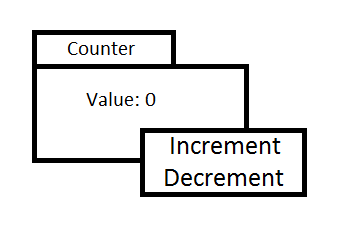
\includegraphics[scale=0.85]{counter.png}
\caption{Kuva CounterView -näkymästä\cite{Krasner:desc}}
\end{figure}

\section{Pyramid}
Pyramid on Python-pohjainen web-sovelluskehys, jonka tehtävänä on helpottaa web-kehitystä tarjoamalla
kehittäjälle valmiita työkaluja avuksi kehitykseen.

\subsection{Tausta}
Sovelluskehyksen tehtävänä on tuoda sovelluksen kehitykseen mukaan
taso, joka tarjoaa erilaisia kirjastoja ratkaisemaan yleisimpiä ongelmia, joita tulee vastaan sovelluksen kehityksen aikana. Näin vältetään
jo ratkaistujen perusoperaatioiden toistoa ja pystytään keskittymään suoraan sovelluksen toteuttamiseen. Web-sovelluskehykset ovat erityisesti suunnattuja
web-sovellusten ja -palvelujen toteuttamiseen\cite{Frameworks}.  Tärkein ero sovelluskehyksen ja kirjaston välillä on se, että kirjaston ohjelmakoodi kutsustaan aina
kehittäjän toimestaa. Sovelluskehyksessä taas kehittäjän ohjelmakoodia kutsutaan aina sovelluskehyksen toimesta\cite{Pyramid:intr}.

\subsection{Sisältö}
Pyramid on suunniteltu siten, että kehittäjän ei tarvitse tietää suuria määriä erilaisia malleja ja tekniikoita pystyäkseen tuottamaan web-sovelluksia. Se ei myöskään pakota käyttämään kehityksessä
mitään erityistä tekniikkaa, vaan pyrkii olemaan mahdollisimman yksinkertainen ja helposti laajennettavissa erilaisiin käyttötarkoituksiin. Laajentamisella tarkoitetaan erilaisten lisäosien
liittämistä Pyramidiin. Yksinkertaisuuden ja mimimaalisuuden ansiosta se on myös nopeampi kuin monet muut Python-pohjaiset web-sovelluskehykset. Tämä johtuu Pyramidin poikkeuksellisen
pienestä kutsupinosta ajamisen aikana\cite{Pyramid:intr}. 

Koska Pyramid pyrkii tarjoamaan vain välttämättömimmät työkalut web-sovelluksien kehitykseen, sen kehittäjät
ovat päätyneet web-kehityksessä neljään yleisimpään ongelmaan ja tarjoavat niihin ratkaisun Pyramidissa:

\begin{description}
\item [URL Mapping] -\ URL:ien liittäminen ohjelmakoodiin.
\item[Template] -\ Tuodaan sovelluksen näkymä selaimelle käyttäen HTML-kuvauskieltä, jolla määrätään näkymän rakenne. Tämän avulla pystytään erottamaan käyttöliittymä sovelluslogiikasta tehokkaasti.
\item[Security] -\ Perinteiset tietoturvaongelmat tulee olla ratkaistuna valmiiksi jo sovelluskehyksessä. Tämä ei kuitenkaan tarkoita sitä, että kehittäjä voisi täysin unohtaa tietoturvan merkityksen.
\item[Static Assets] -\ Staattisien resurssejen jakaminen niille tarkoitettuihin paikkoihin tiedostorakenteessa.
\end{description}
Yllä määriteltyjen neljän pääongelman lisäksi Pyramid tarjoaa lisäosien kautta monia erilaisia työkaluja, joiden avulla pystytään laajentamaan sen ominaisuuksia\cite{Pyramid:intr}. Tutkielman aiheen rajauksen vuoksi ei kuitenkaan
käydä läpi yksityiskohtaisemmin Pyramidin toteutusta ja siihen liitettävissä olevia lisäosia, vaan keskitytään tarkastelemaan MVC:n toteutusta Pyramidissa.

\subsection{Tiedostorakenne}
Kuten monissa web-sovelluskehyksissä, jaetaan sovelluslogiikka erillisiin tiedostoihin. Näin jokaisella ohjelmakoodilla on oma paikkansa ja sovelluksen hallinta kehityksen aikana helpottuu. Samalla
sovelluskehys löytää tarvittavat asiat oikeista paikoista. Pyramidissa ei kuitenkaan pakoteta ohjelmakoodia mihinkään tietynnimiseen tiedostoon. Esimerkiksi mallin ohjelmakoodin ei tarvitse olla \emph{models.py} -tiedostossa, vaan sen voi määritellä myös muualla. Tässä tutkimuksessa käytämme kuitenki  tiedostorakennetta, joka generoidaan Scaffold työkalulla\cite{scaffold}. Scaffoldilla voidaan luoda valmiita tiedostorakenteita, jotka sisältävät kaikki tarvittavat osat sovelluksen rakentamiseen. Seuraavassa kuvassa esitellään yksinkertaisen web-sovelluksen rakenne Pyramidissa: \\

\Tree  [.Sovellus !\qsetw{0.6pt} [ kuva.png tyyli.css ].static  [ template.pt ].templates \_\_init\_\_.py views.py models.py ] \\

Ilman tiedostopäätettä olevat lehdet ovat kansioita, jotka sisältävät muita tiedostoja. Tiedostot \emph{models.py}, \emph{views.py} ja \emph{\_\_init\_\_.py} ovat Python-moduuleita, jotka sisältävät
sovelluksen ohjelmakoodin. Yksinkertaistettuna \emph{\_\_init\_\_ .py}:ssä alustetaan sovellus. Pyramidissa näkymien ohjelmakoodi on yleensä määritelty \emph{views.py} -tiedostossa ja
mallit luodaan \emph{models.py} -tiedostossa. Kyseiset tiedostot eivät kuitenkaan sisällä mitään riippuvuuksia malleihin tai näkymiin. On kuitenkin suositeltavaa, että ohjelmakoodi jaotellaan tiedostokohtaisesti malleihin ja näkymiin. Kansion \emph{static} sisällä ovat kaikki staattiset resurssit, joita käytetään sovelluksessa. Staattisia resursseja voivat olla esimerkiksi kuva-, ääni- tai tyylitiedostot.
Kansion \emph{templates} alta löytyvät kaikki \emph{template}-tiedostot, jotka määräävät sovelluksen näkymän selaimessa. Templatet yhdistävät selaimille tarkoitetun HTML-kuvauskielen sekä ohjelmakoodin yhtenäiseksi dokumentiksi, joka tuodaan selaimelle näytettäväksi. Tässä tutkielmassa mielenkiinto on kohdistettu \emph{views.py}, \emph{models.py} ja \emph{template.pt}
-tiedostoihin, koska ne sisältävät tarvittavat toteutukset MVC:n tarkasteluun.

Alla on lyhyt selvitys MVC:n kannalta oleellisten tiedostojen sisällöstä:
\begin{description}
\item [views.py] \ Nimensä mukaisesti sisältää näkymien ohjelmakoodin, jotka liitetään \emph{template}-tiedostoihin.
\item[template.pt] \ Tuodaan sovelluksen näkymä selaimelle käyttäen HTML-kuvauskieltä, jolla määrätään näkymän rakenne. Tämän avulla pystytään erottamaan käyttöliittymä sovelluslogiikasta tehokkaasti.
\item[models.py] \ Sisältää mallejen ohjelmakoodit.
\end{description}

\section{MVC \& Pyramid}
Pyramidin kehittäjien dokumenteissa esitellään Pyramid MVC-kehyksenä, mutta samalla myös kyseenalaistetaan tämä väite. Erityisesti mallin ja ohjaimen määritelmä puuttuu\cite{Pyramid:intr}. Tässä
osiossa käsitellään Pyramidia MVC:n näkökulmasta. 

\subsection{Näkökulman rajaaminen}
Tutkielmassa keskitytään Pyramidin alkuperäiseen toteutukseen, joten lisäosien tarjoamiin erilaisiin tekniikoihin ja toteutuksiin oteta kantaa. Tämä on tutkielman kannalta tärkeää, koska kaikkien
mahdollisten lisäosien tuomien tekniikoiden tutkiminen olisi lähes mahdotonta. Näin tutkielma pysyy myös kandidaatin tutkielman rajoissa.

Pyramidin sovellusarkkitehtuuri on toteutettu käyttäen pohjana MVC-arkkitehtuuria. Tämä ei kuitenkaan tarkoita sitä, että Pyramid toteuttaisi MVC:n teknisesti sellaisena kuin esimerkiksi Krasner määrittelee\cite{Krasner:desc}. Teknisyydellä
tarkoitetaan tässä kontekstissa tarkkoja ohjelmointiteknisiä ratkaisuja, jotka ovat sidottuja tiettyyn kieleen tai työkaluun. Web-ohjelmointi tuo itsessään jo rajoituksia MVC-komponenttien kommunikaatiolle
Pyramidissa. Esimerkiksi pyyntö tulee suorittaa aina, jos palvelimelta halutaan tuoda dataa selaimelle\cite{Web}. Tämän perusteella malli ei voi viestittää muutoksestaan näkymälle ja ohjaimelle ilman niiden kautta tulevaa pyyntöä toisinkuin esimerkiksi Krasnerin määritelmässä\cite{Krasner}. Ohjelmointityökalujen määrän sekä vauhdikkaan kehityksen myötä tämä voidaan kuitenkin mahdollisesti kiertää tulevaisuudessa. Tästä syystä MVC-toteutusta ei ole tutkielman kannalta järkevää tutkia liian teknisestä näkökulmasta, vaan toteutusta tulee tarkastella korkeammalla tasolla. Tässä osiossa oletetaan MVC:n olevan abstrakti malli ohjelmakoodin jakamiselle helposti hallittaviin osiin. Se kuinka tämä teknisesti toteutetaan ei ole tutkielman kannalta oleellista.
Koska MVC:n toteutusta Pyramidissa tarkastellaan abstraktilla tasolla, määritetään selkeät ominaisuudet, jotka MVC-komponenttien tulee toteuttaa. Jokaisen komponentin on toteutettava sille määrätyt ominaisuudet, jotta voidaan todeta sen kuuluvan osaksi MVC-arkkitehtuuria. Ominaisuudet määritellään käyttäen pohjana Burbeckin ja Krasnerin julkaisuja\cite{Burbeck, Krasner:desc}.

Tärkeimpänä vaatimuksena on se, että näkymä ja ohjain luovat rajapinnan, jonka kautta käyttäjä keskustelee mallin kanssa. Malli ei saa olla suorassa yhteydessä käyttäjään\cite[s. 10]{Reenskaug:tools}.
Mallin tulee olla riippumaton näkymästä ja ohjaimesta. Sen tulee myös hallita sovelluksen tilaa sekä pystyä antamaan informaatiota sovelluksen tilasta\cite{Burbeck}. Näkymän on keskusteltava mallin kanssa sekä hoitaa mallilta saadun datan graafinen näyttäminen\cite[s.1]{Reenskaug:orig}. Ohjain puolestaan ottaa vastaan syötteitä ja lähettää viestejä tämän perusteella näkymälle ja mallille\cite{Burbeck}. Näiden rajoituksien perusteella pystytään vastaamaan tutkimuksessa siihen, toteuttaako Pyramid MVC-arkkitehtuurin vai ei.

Tarkastelua varten toteutetaan Pyramidilla vastaava laskurisovellus kuin Krasnerin julkaisussa käyttäen Pyramidin tarjoamia ominaisuuksia\cite{Krasner:desc}. Sovellus rajataan käyttämään SQL-tietokantaa mallin datan tallennukseen sekä \emph{URL dispatch} -tekniikkaa\cite{urldispatch, sql}. Sovelluksen pohjalta tarkastellaan MVC:n kannalta kolmea oleellisinta tiedostoa: \emph{views.py}, \emph{models.py} ja \emph{template.pt}. Näin tutkimuksen tarkastelu pystytään rajaamaan mahdollisimman pienelle alueelle, jolloin tutkimus on helpompi keskittää tarkastelemaan yksittäistä tekniikkaa. Samalla tutkimus pysyy myös kandityön rajoisssa. Kaikkea sovelluksen sisältämää ohjelmakoodia ei käydä läpi, vaan tiedostoista otetaan esiin vain MVC:n kannalta oleellisin ohjelmakoodi.

Tässä osiossa tarkastellaan Pyramid-sovelluksen tiedostoja sekä niiden sisältöjä MVC-komponentteina. Erityisesti keskitytään ohjaimen ja näkymän toteukseen. Samalla tutkitaan voidaanko Pyramid havaintojen perusteella luokitella MVC:n toteuttavaksi sovelluskehykseksi.
Koska Pyramidissa MVC-arkkitehtuurin määrittely on hyvin epävakaalla pohjalla, tulee tehdä selkeä oletus komponentteien jaottelulle. Esimerkiksi \emph{views.py} ja \emph{template.pt} -tiedostot ovat tarkoitettu toimimaan yhdessä näkymänä, jolloin ohjaimen toteuttamat tehtävät sisällytettäisiin näkymään. MVC:tä tutkiessa täytyy sovelluksen komponentit kuitenkin jakaa kolmeen osaan.  Tiedosto \emph{views.py}
sisältää paljon ohjaimelle yhteisiä piirteitä, joten se erottuu selvästi \emph{template.pt} -tiedostosta. Tutkimuksessa oletetaan, että \emph{models.py} sisältää mallin, \emph{views.py} ohjaimen ja \emph{template.pt} näkymän.

\subsection{Tiedostojen tarkastelu}
\lstset{
  literate={ö}{{\"o}}1
           {ä}{{\"a}}1,
xleftmargin=30pt,
escapeinside={/*@}{@*/},
backgroundcolor=\color{light-gray}
}
\lstset{numbers=left}
\begin{lstlisting}[language=Python]
# Tiedosto: models.py
class Counter(Base):
    __tablename__ = 'counter'

    # Asetetaan mallille atribuutit, jotka
    # vastaavat mallin tilasta.
    id = Column(Integer, primary_key=True)
    name = Column(Unicode(255), unique=True)
    value = Column(Integer)

    # Määritellään luokalle konstruktori,
    # joka saa parametreiksi nimen ja alkuarvon.
    def __init__(self, name, value):
        self.name = name
        self.value = value

    def increment(self):
        self.value += 1

    def decrement(self):
        self.value -= 1

# Luodaan instanssi mallista ja rekisteröidään 
# se sovellukseen.
def populate():
    session = DBSession()
    model = Counter(name=u'counter', value=0)
    session.add(model)
\end{lstlisting}

\emph{Models.py} -tiedosto sisältää malliin liittyvän ohjelmakoodin. Jokaiselle mallille luodaan aina oma luokkansa, jossa määritellään mallin ominaisuudet. Malli rekisteröidään \emph{populate()} -metodin kautta, jota kutsutaan Pyramidin toimesta.
Ohjelmakoodista nähdään, että malli ei luo minkäänlaista riippuvuutta näkymään tai ohjaimeen. Se myös pitää huolen datan käsittelystä.  Malli on siis Pyramidissa itsenäinen komponentti, joka huolehtii sovelluksen tilasta. Tämän perusteella malli toteutuu Pyramidissa MVC-arkkitehtuurin mukaisesti. \\

\emph{Views.py} -tiedostossa määritellään näkymän ohjelmakoodi. Pyramidissa on konkreettisesti määritelty ohjelmakooditasolla vain malli ja näkymä.
Jokaista näkymää kohden on oma funktio, joka ottaa vastaan \emph{request} -olion. Request-oliossa tuodaan sovellukselle kaikki tieto käyttäjästä ja sovelluksen viesteistä. Tämän perusteella tulkitaan request-oliossa tuotu data käyttäjän syötteiksi.
Vaikka \emph{views.py} nimetään Pyramidissa näkymäksi, on se toteutukseltaan hyvin lähellä ohjainta. Tästä syystä tarkastellaan funktion toteutusta mahdollisena ohjaimena. Tästä eteenpäin puhutaessa ohjaimesta Pyramidissa, tarkoitetaan sillä \emph{views.py} -tiedoston sisältämää funktiota.

\lstset{
  literate={ö}{{\"o}}1
           {ä}{{\"a}}1,
xleftmargin=30pt,
escapeinside={/*@}{@*/},
}
\begin{lstlisting}[language=Python]
# Tiedosto: views.py
@view_config(route_name='counter_view',
	renderer='templates/counter.pt')
def counter_view(request):
    dbsession = DBSession()

    # Rekisteröidään malli.
    counter = dbsession.query(Counter).filter(
	Counter.name==u'counter').first()
    try:
        request.params['minus'].
        counter.decrement()
    except KeyError:
        pass

    try:
        request.params['plus']
        counter.increment()
    except KeyError:
        pass

    # Palautetaan laskurin arvo, joka tulkitaan
    # ja näytetään template.pt -tiedostssa
    return {'value': counter.value}
\end{lstlisting}

Määritellään funktiolle URL-osoite sekä liitetään siihen template -tiedosto (2). Tämän jälkeen rekisteröidään malli mukaan funktioon (8). Koska tarkastelemme funktiota ohjaimena, voimme tulkita templaten näkymäksi. Tällöin funktioon rekisteröidään malli sekä näkymä, jolloin rekisteröinnin puolesta se toteuttaa ohjaimen MVC:ssä.
Funktioon lisätään myös toiminto laskurin vähentämiselle. Mallin emph{value} -arvoa muutetaan, kun request-oliosta löytyy tietty parametri. Funktio palauttaa paluuarvona mallin arvon, joka tuodaan käsiteltäväksi templateen. Funktio siis ottaa vastaan syötteitä ja niiden perusteella lähettää lähettää viestejä
mallille sekä näkymälle. Tämän perusteella todetaan, että se täyttää rajauksessa määrätyt ohjaimen ominaisuudet. \\

Templatessa yhdistetään HTML-merkkauskieli ja sovelluksen ohjelmakoodi. Tästä generoidaan HTML-sivu, joka näytetään selaimelle. Koska malli sekä ohjain on jo määritelty, täytyy selvittää täyttääkö template näkymälle määritellyt ominaisuudet.
\begin{lstlisting}[language=Python]
  <body>
    <h1>${value}</h1>
    <form action="./" method="get">
      <button type="submit" name="plus" value="plus">
		Increment </button>
      <button type="submit" name="minus" value="minus"> 
		Decrement </button>
    </form>
  </body>
\end{lstlisting}
Templatessa luodaan lomake kahdelle painikkeelle, joista kumpikin lähettää lomakkeen eteenpäin \emph{counter\_view} -funktiolle. Lomakkeen tiedot tulevat funktiolle request-oliossa, joka sisältää tässä tapauksessa \emph{plus}- tai \emph{minus}-parametrin riippuen siitä kumpaa painiketta on painettu. Lomakkeen tiedot lähetetään samaan osoitteeseen (3), mistä sitä on alunperin kutsuttukin. Eron tuo kuitenkin request-oliossa tuodut parametrit.  Otsikossa (2) tuodaan näkyviin laskurin sen hetkinen arvo, joka saadaan tietoon ohjaimelta.
 Templatessa hoidetaan sovelluksen graafinen puoli, joten se vastaa osaltaan näkymää. \\ Ongelmaksi muodostuu kuitenkin näkymän ja mallin välinen kommunikointi. Näkymä ei ole yhteydessä malliin suoraan, vaan tarvitsee ohjaimen kautta tiedon mallin tilasta.  Näkymä ei siis sellaisenaan toteuta sille asetettuja ominaisuuksia. \\

\subsection{Sovelluksen toiminta}
Alla olevassa kuvassa esitellään visuaalisesti miten laskurisovellus muodostaa HTML-sivun, kun käyttäjä painaa sivulla \emph{Increment} -painiketta. Kuvan
vaiheet toteutetaan numerojärjestyksessä alkaen ensimmäisestä.
\begin{figure}[h]
\centering
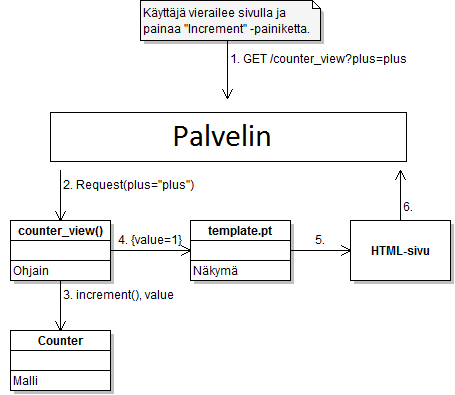
\includegraphics[scale=0.87]{laskurisovellus.png}
\caption{Laskurisovelluksen toiminta}
\end{figure}
\lstset{
  literate={ö}{{\"o}}1
           {ä}{{\"a}}1,
xleftmargin=30pt,
escapeinside={/*@}{@*/},
}

\begin{lstlisting}
/*@Palvelimelta pyydetään HTTP-protokollan mukaisesti sivua \emph{plus} -parametrilla.@*/
/*@Palvelin pyytää sovellukselta sivua. Parametri tuodaan sovellukselle \emph{request}-oliossa.@*/
/*@Ohjain käskee mallia muuttamaan tilaansa ja pyytämään samalla tiedon muutoksen jälkeisestä arvosta.@*/
/*@Ohjain palauttaa mallin arvon, joka käsitellään templatessa.@*/
/*@Templatessa generoidaan HTML-sivu, joka tuodaan palvelimelle vastauksena.@*/
\end{lstlisting}

\subsection{Yhteenveto}
Malli sekä ohjain toteutuvat Pyramidissa MVC:n mukaisesti. Malli on itsenäinen komponentti, jolla ei ole riippuvuutta näkymään tai ohjaimeen. Se myös huolehtii sovelluksen käsittelemästä datasta ja vastaa tarvittaviin pyyntöihin. Ohjain taas huolehtii request-oliossa tulevista syötteistä ja vaikuttaa malliin sekä näkymään.  Kumpikin edellä mainittu komponentti toteuttaa MVC:ssä sille tarkoitetun roolin. Näkymä toteuttaa sovelluksen graafisen näyttämisen selaimelle, mutta ei toteuta sille määrättyjä sääntöjä. MVC:ssä näkymän tarkoitus on kommunikoida suoraan mallin kanssa. Tämä ei kuitenkaan onnistu Pyramidissa, jossa näkymä on yhteydessä vain ohjaimeen.

\section{Tulokset}
Pyramidin MVC-toteutusta tarkastellessa tulee ottaa huomioon yksittäisien komponenttien toteutus sekä niiden välinen yhteistyö. Yksittäiset komponentit toteutuvat Pyramidissa MVC-arkkitehtuurin mukaisesti, mutta niiden välinen yhteistyö
toteutetaan eri tavalla. Erityisesti näkymäksi erotettu template tuo ongelmia, koska se ei suoraan yhteydessä mallin kanssa. 

Pyramidin MVC-komponenttien kommunikointi voidaan esittää käyttäen pohjana muokaten Krasnerin kommunikaatiomallia\cite{Krasner:desc}.
Alla esitellyssä kuvassa havainnollisestetaan, kuinka mallin ja näkymän kommunikaatio puuttuu täysin ja kaikki data tuodaan ohjaimen kautta.

\begin{figure}[h]
\centering/
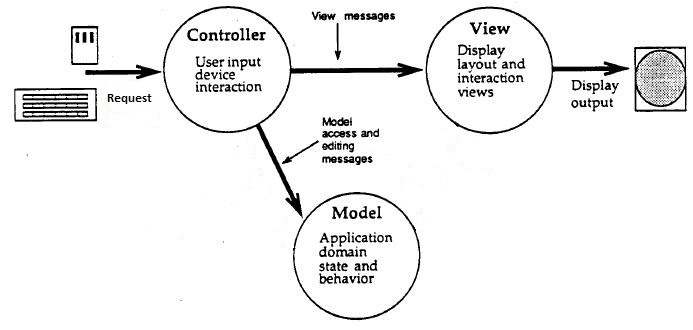
\includegraphics[scale=0.85]{pyramid_mvc.jpg}
\caption{Pyramidin kommunikointi MVC-komponenttien kesken. Kuva on muokattu Krasnerin esittelemästä kommunikointimallista\cite{Krasner:desc}  }
\end{figure}

Yllä esitetyssä kommunikaatiomallissa ohjain saa vastaan request-olion, jossa tuodaan kaikki tarvittava tieto käyttäjästä. Tämän perusteella ohjain ohjaa mallia
sekä muuttujaa. Samalla se pyytää mallilta tietoa sovelluksen tilasta ja välittää tiedon näkymälle. Näkymä taas välittää ohjaimen tuoman datan käyttäjälle graafisena.

\section{Johtopäätökset}
Web-sovellusten toteutus tuo suoraan rajoitteita MVC-arkkitehtuurin toteutukselle. Erityisesti ongelmaksi muodostuu mallin viestiminen muutoksesta, koska kaikki data haetaan selaimen pyynnön kautta. Samalla MVC:n alkuperäisessä julkaisussa määrätään, että näkymä ei saa olla missään tekemisissä käyttäjän syötteiden kanssa\cite[s. 1]{Reenskaug:orig}. Esimerkiksi hiiren valinnat sekä näppäimistön syötteet tulisivat aina ohjaimen kautta. Tämä ei kuitenkaan ole Pyramidissa mahdollista, koska monissa tapauksissa syötteet tulevat selaimen kautta
templaten generoiman HTML-sivun avulla. Syötteet tulee siis rajata request -olion sisältämään dataan.
Tästä syystä MVC:tä ei ole järkevää tarkastella liian teknisestä näkökulmasta, vaan rajata tarkastelu korkeammalle tasolle.

Alunperin Pyramidin dokumentaatiossa kyseenalaistettiin mallin sekä ohjaimen toteutus\cite{Pyramid:intr}. Tutkimuksen pohjalta voidaan kuitenkin
todeta, että ongelmaksi ei muodostu yksittäisien komponenttien toteutus, vaan komponenttien välinen kommunikointi. Erityisesti näkymän ja mallin yhteistyö jää
kokonaan puuttumaan, jolloin saadaan ristiriita MVC:n alkuperäisen määritelmän kanssa\cite[s. 1]{Reenskaug:orig}. Tämä johtuu siitä, että Pyramidissa \emph{views.py} -tiedoston sisältämä ohjelmakoodi on nimensä mukaisesti tarkoitettu näkymäksi ja
\emph{template.pt} -tiedosto katsotaan osaksi samaa komponenttia. Tutkimuksen tuloksien perusteella voidaan kuitenkin todeta, että \emph{views.py} -tiedoston näkymä-funktio toteuttaa kaikki
ohjaimelle määritellyt ominaisuudet. Template puolestaan hoitaa sovelluksen graafisen puolen, joten sen ominaisuudet ovat mahdollisimman lähellä näkymää. Template ei kuitenkaan riitä toteuttamaan näkymän ominaisuuksia, koska se on täysin riippuvainen ohjaimesta. 

Vaikka MVC:n toteutusta tutkitaan hyvin abstraktilla tasolla, ei Pyramid toteuta MVC-arkkitehtuuria. Pyramidissa näkymä ja ohjain on yhdistetty yhteen komponenttiin, joka kommunikoi mallin kanssa. Näitä komponentteja ei pystytä kuitenkaan erottamaan toisistaan siten, että MVC-arkkitehtuuri toteutuisi. Tutkielman pohjalta voimme määritellä Pyramidin käyttävän MVC-arkkitehtuurin pohjalta toteutettua muunnosta, jossa kommunikaatiomallia on muutettu ja ohjain on sisällytetty näkymään. 

\begin{thebibliography}{13} % alle 15 lähdeteosta
\bibitem{Deacon:1995}
    John Deacon Computer Systems Development, Consulting \& Training
    \emph{Model-View-Controller (MVC) Architecture},
    August 1995, revised August 2000, April 2005 and May 2009

\bibitem{Burbeck}
   Burbeck Steve, 1992
  \emph{“Applications Programming in Smalltalk-80(TM): How to use Model-View-Controller (MVC)”,}
  \url{http://st-www.cs.illinois.edu/users/smarch/st-docs/mvc.html}

 \bibitem{Krasner}
   Glenn E. Krasner \& Stephen T. Pope, 1988
  \emph{“A Cookbook for Using the Model-View-Controller User Interface Paradigm in Smalltalk-80”,}
  \url{http://www.ics.uci.edu/~redmiles/ics227-SQ04/papers/KrasnerPope88.pdf}

\bibitem{Krasner:desc} 1988 Glenn E. Krasner \& Stephen T. Pope, ParcPlace Systems Inc,
	\emph{"A Description of the Model-View-Controller User Interface Paradigm in the Smalltalk-80 System"}
	\url{http://www.create.ucsb.edu/~stp/PostScript/mvc.pdf}

 \bibitem{Reenskaug}
  XEROX PARC 1978-79
  \emph{MVC XEROX PARC 1978-79}
http://heim.ifi.uio.no/~trygver/themes/mvc/mvc-index.html

 \bibitem{Reenskaug:1979}
  XEROX PARC 1979
  \emph{THING-MODEL-VIEW-EDITOR}
   http://heim.ifi.uio.no/~trygver/1979/mvc-1/1979-05-MVC.pdf

 \bibitem{Reenskaug:2007}
  XEROX PARC 1979
  \emph{The Original MVC reports}
 \url{http://heim.ifi.uio.no/~trygver/2007/MVC_Originals.pdf}

 \bibitem{Reenskaug:orig}
  Trygve Reenskaug 1979
  \emph{Models-Views-Controllers}
 \url{http://heim.ifi.uio.no/~trygver/1979/mvc-2/1979-12-MVC.pdf}

\bibitem{Reenskaug:tools}
 \emph{The Model-View-Controller (MVC) Its Past and Present}
\url{http://heim.ifi.uio.no/~trygver/2003/javazone-jaoo/MVC_pattern.pdf}

 \bibitem{Pyramid:intr}
  \emph{Pyramid Introduction}
   \url{http://www.kemeneur.com/clients/pylons/docs/pyramid/narr/introduction.html}

\bibitem{Web}
\emph{Research on Web Instant Messaging Using REST Web Service}
http://ieeexplore.ieee.org/stamp/stamp.jsp?arnumber=05607397

\bibitem{Sqlalchemy}
\emph{Sqlalchemy}
www.sqlalchemy.org

\bibitem{urldispatch}
\emph{Pyramid Documentation, URL Dispatch}
\url{http://docs.pylonsproject.org/projects/pyramid/en/latest/narr/urldispatch.html}

\bibitem{mvcframeworks}
bestwebframeworks 2009
\emph{List of Python MVC-frameworks by bestwebframeworks.com}
http://www.bestwebframeworks.com/compare-web-frameworks/python/

\bibitem{scaffold}
Pyramid Documentation
\emph{Creating Pyramid Scaffolds}
http://docs.pylonsproject.org/projects/pyramid/en/latest/narr/scaffolding.html

\bibitem{sql}
W3Schools.com, 1999-2012 Refsnes Data
\emph{Introduction to SQL}
\url{http://www.w3schools.com/sql/sql_intro.asp}

\bibitem{ZCA}
2007-2009 Baiju M
\emph{A Comprehensive Guide to Zope Component Architecture}
\url{http://www.muthukadan.net/docs/zca.pdf}

\bibitem{grok}
2007-2008, The Grok Community
\emph{Grok: About}
\url{http://grok.zope.org/about/}

\bibitem{zope}
2012 Zope Foundation
\emph{Zope Website}
\url{http://www.zope.org}

\bibitem{URL}
T. Berners-Lee CERN L. Masinter Xerox Corporation M. McCahill, University of Minnesota December 1994
\emph{Uniform Resource Locators (URL)}
\url{http://www.ietf.org/rfc/rfc1738.txt}

\bibitem{HTML}
Dave Raggett, W3C Recommendation 14-Jan-1997
\emph{HTML 3.2 Reference Specification}
\url{http://www.w3.org/TR/REC-html32}


\end{thebibliography}
\end{document}
